\documentclass[21pt,a4paper,notitlepage]{report}
\renewcommand{\thesection}{\arabic{section}}


\usepackage {url}
\usepackage [numbers]{natbib}
\usepackage[T1]{fontenc}
\usepackage[utf8]{inputenc}
\usepackage{lmodern}
\usepackage{setspace}
\usepackage{amsfonts}
\usepackage{graphicx}
\usepackage{listings}
\usepackage{CJKutf8}
\lstset{basicstyle=\footnotesize, breaklines=true}
%\usepackage[a4paper,left=2.5cm,right=2.5cm,top=2.5cm,bottom=2.5cm]{geometry}

\usepackage{makecell}

\begin{document}
  \begin{titlepage}
\centering
Bogazici University Computer Engineering Department\\
CMPE 58H Team Project\\
\vspace*{11\baselineskip}
\LARGE
\bfseries
Druggy \\ Drug - Adverse Effect Website\\[2\baselineskip]
\normalfont
\footnotesize
\small
\vfill
Team - O \\ \{dilara.kekulluoglu,mesut.keskin,\\ yasemin.yenigun,nebih.basaran\}@boun.edu.tr \\[3\baselineskip]


\textbf{\today} \\[2\baselineskip]
\end{titlepage}

\section*{Abstract}
We use social media everyday for different
reasons. The variety is astonishing, people
can share pictures, meet with like-minded people,
share videos and so on. In this project we
are creating a social semantic website
that users search for adverse effects of
drugs and also enter such information themselves.

\section{Introduction \& Motivation}
\label{sec:intro}
We have done a project named Druggy for the term project which is a
requirement of Cmpe58H Social Semantic Web course.
Drugs have been used for years to heal people's illnesses.
They are produced and manufactured by companies in many different
names. Even countries have different drugs for the same purpose.
For example Majezik in Turkey which is for head ache is
named as Ocufen in United States. Since they have
many different names, it is hard to search for adverse
effects online. Prospectuses of drugs are obligated to contain information
about adverse effects. However, this info is often hard
to understand. Also the experienced effects by real users
might differ according the features of a user.

In addition, information providers are increasingly
inclined to give false information or exaggerated
information to gain popularity in the internet environment.
Due to this, the difficulty of obtaining accurate information
on drugs is increasing day by day. In our Druggy project, we have
set up a platform to provide both formal and informal information
on drugs to the people who use drugs or want to learn about them.
With its social and semantic features, this platform is both a social 
area for drug users and a platform for accurate information about drugs.
Druggy is a self-improving platform that increases its knowledge
every time by using the data from the user input.
In Druggy project, users are allowed to search drugs,
see the adverse effects from both formally approved information
and the data that is generated from user inputs.

\section{General Framework}
\subsection{Formal Semantic Data From Sider}
As we mentioned in introduction, Druggy is a platform that
brings together formal information. In order to provide this feature,
Sider~\cite{sider}, a fully approved medication platform with formal information,
was used. Our goal here is to provide information about the drugs together with all the details. For this reason, the side effects of the drugs, the parts that they affect on the body and their ingredients are taken from the Sider platform. A sample taken data is as follows.

\begin{table}
	\vskip\baselineskip 
	\begin{center}
		{\caption{Information Adding From SIDER}}
		\resizebox{\textwidth}{!}{%
			\begin{tabular}{ | c | c | c | c |}
				\hline
			 \thead{Drug Name} &  \thead{Ingredient}  & \thead{Adverse Effect}  &   \thead{Body Part}\\ \hline
			
				Parol  & Acetominophen &  \makecell{Diarrhoea\\ Dizziness \\ Headache }
				 & \makecell{ Bowel \\	 Eyes \\ Head\\ Stomach} \\	\hline		
			\end{tabular}%
		}
	\end{center}
\end{table}

In order to be able to test the platform in the first place, approximately 20 drugs were added to the system in full detail. The added drugs were selected among the most commonly used drugs in the society. 

In addition to the taken data, a description has been added for each adverse effect in order to allow users to have system’s suggestions when they are looking for a drug, adverse effect, ingredient or body part.  

\subsection{Functionality}
The diagram for search and adding new entries can be seen in Figure~\ref{fig:use}.

\begin{figure}
	\centering
	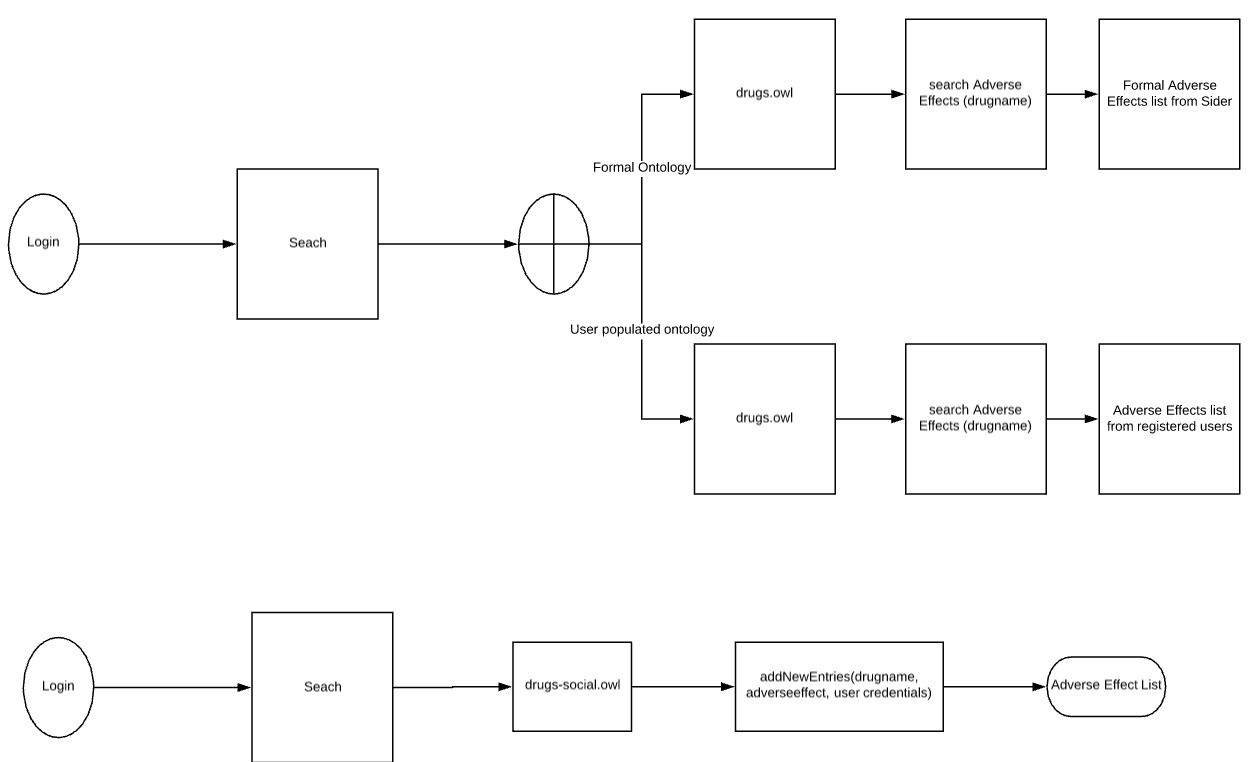
\includegraphics[width=0.8\textwidth]{use.png}
	\caption{Diagram for User Interactions}
	\label{fig:use}
\end{figure}

\begin{itemize}
	\item \textbf{search.py} : The class for extracting data from the formal ontology. It uses ontologyHandler for getting data from the ontology.
	Ontology manipulation is done with owlready2~\cite{owlready} in this class.
	It gets adverse effects for drugs and vice-versa. Also if you give it a phrase,
	it can return the most possible adverse effects that match that phrase.
	\item \textbf{search\_social.py} : The ontology handler for user-generated ontology. It considers the credentials of the user when searching the ontology.
	The search is done with rdflib~\cite{rdflib} using SPARQL queries.
	\item \textbf{addEntries.py} : As the name suggests, this class gets drug,
	adverse effect and user credentials and creates a new entry for the user-generated ontology. This also uses ~\cite{owlready} for ontology handling.
	\item \textbf{recommendTags.py} : After a user enters a blog, this class
	is called for smart tag recommendation. User might not enter the tags correctly. This class takes a string and returns possible tags from the formal ontology.
\end{itemize}



\section{Simulation Data}
A simulation data set was created to test the platform features efficiently. All data in this dataset has been generated. This dataset allowed us to model the results according to the user’s age, gender, height, weight etc. An example of the data is as follows;

\begin{figure}
	\centering
	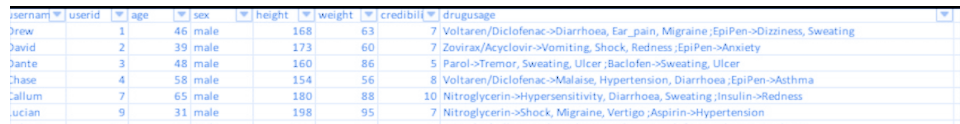
\includegraphics[width=0.8\textwidth]{data.png}
	\caption{Simulation Data}
	\label{fig:data}
\end{figure}

The data shown in the above table represents the following information of the users.
\begin{itemize}
	\item Username: The username that user chooses to login the platform
	\item Userid: The id given automatically by the system to the user.
	\item Age: User’s age
	\item Sex: User’s gender
	\item Height: User’s height
	\item Weight: User’s weight
	\item Drugusage: User’s drug history
	\item Credibility: User’s trust score
\end{itemize}

Drugusage column indicates which drug user is using and side effects from that drug. For example for user David, he uses Zovirax/Acyclovir which has Vomiting, Shock, Redness as adverse effects and Epipen which has Asthma as adverse effect. This column helps us to model the data and show more accurate data according to the user’s information. In addition to that we have added “credibility” column which shows user’s trust score.Simulation data contains information of more than 100 individuals in total.This is a sufficient data for the system to work and to test every feature.

\section{Example}
Dilara has been suffering from cramping occasionally in her footsteps she thinks that mighy be because of aspirin and Xanax drugs  that she has been using for a month. Dilara wants to satisfy their curiosity, decides to search the side effects of aspirin and Xanax on Draggy. Dilara did not see the cramp in side effects when she searched Aspirin on the platform.That was not surprising. Because her mother swore that aspirin could not cause cramps.When she searched for Xanax, Dilara saw that cramp was a side effect of Xanax, even if it was really low. After seeing this, Dilara decided to add cramps as a side effect of Xanax because she knew that Druggy is an user a populated platform. After doing the insert, Dilara saw what she wrote in Xanax’s results in the user contributions section.

\begin{figure}
	\centering
	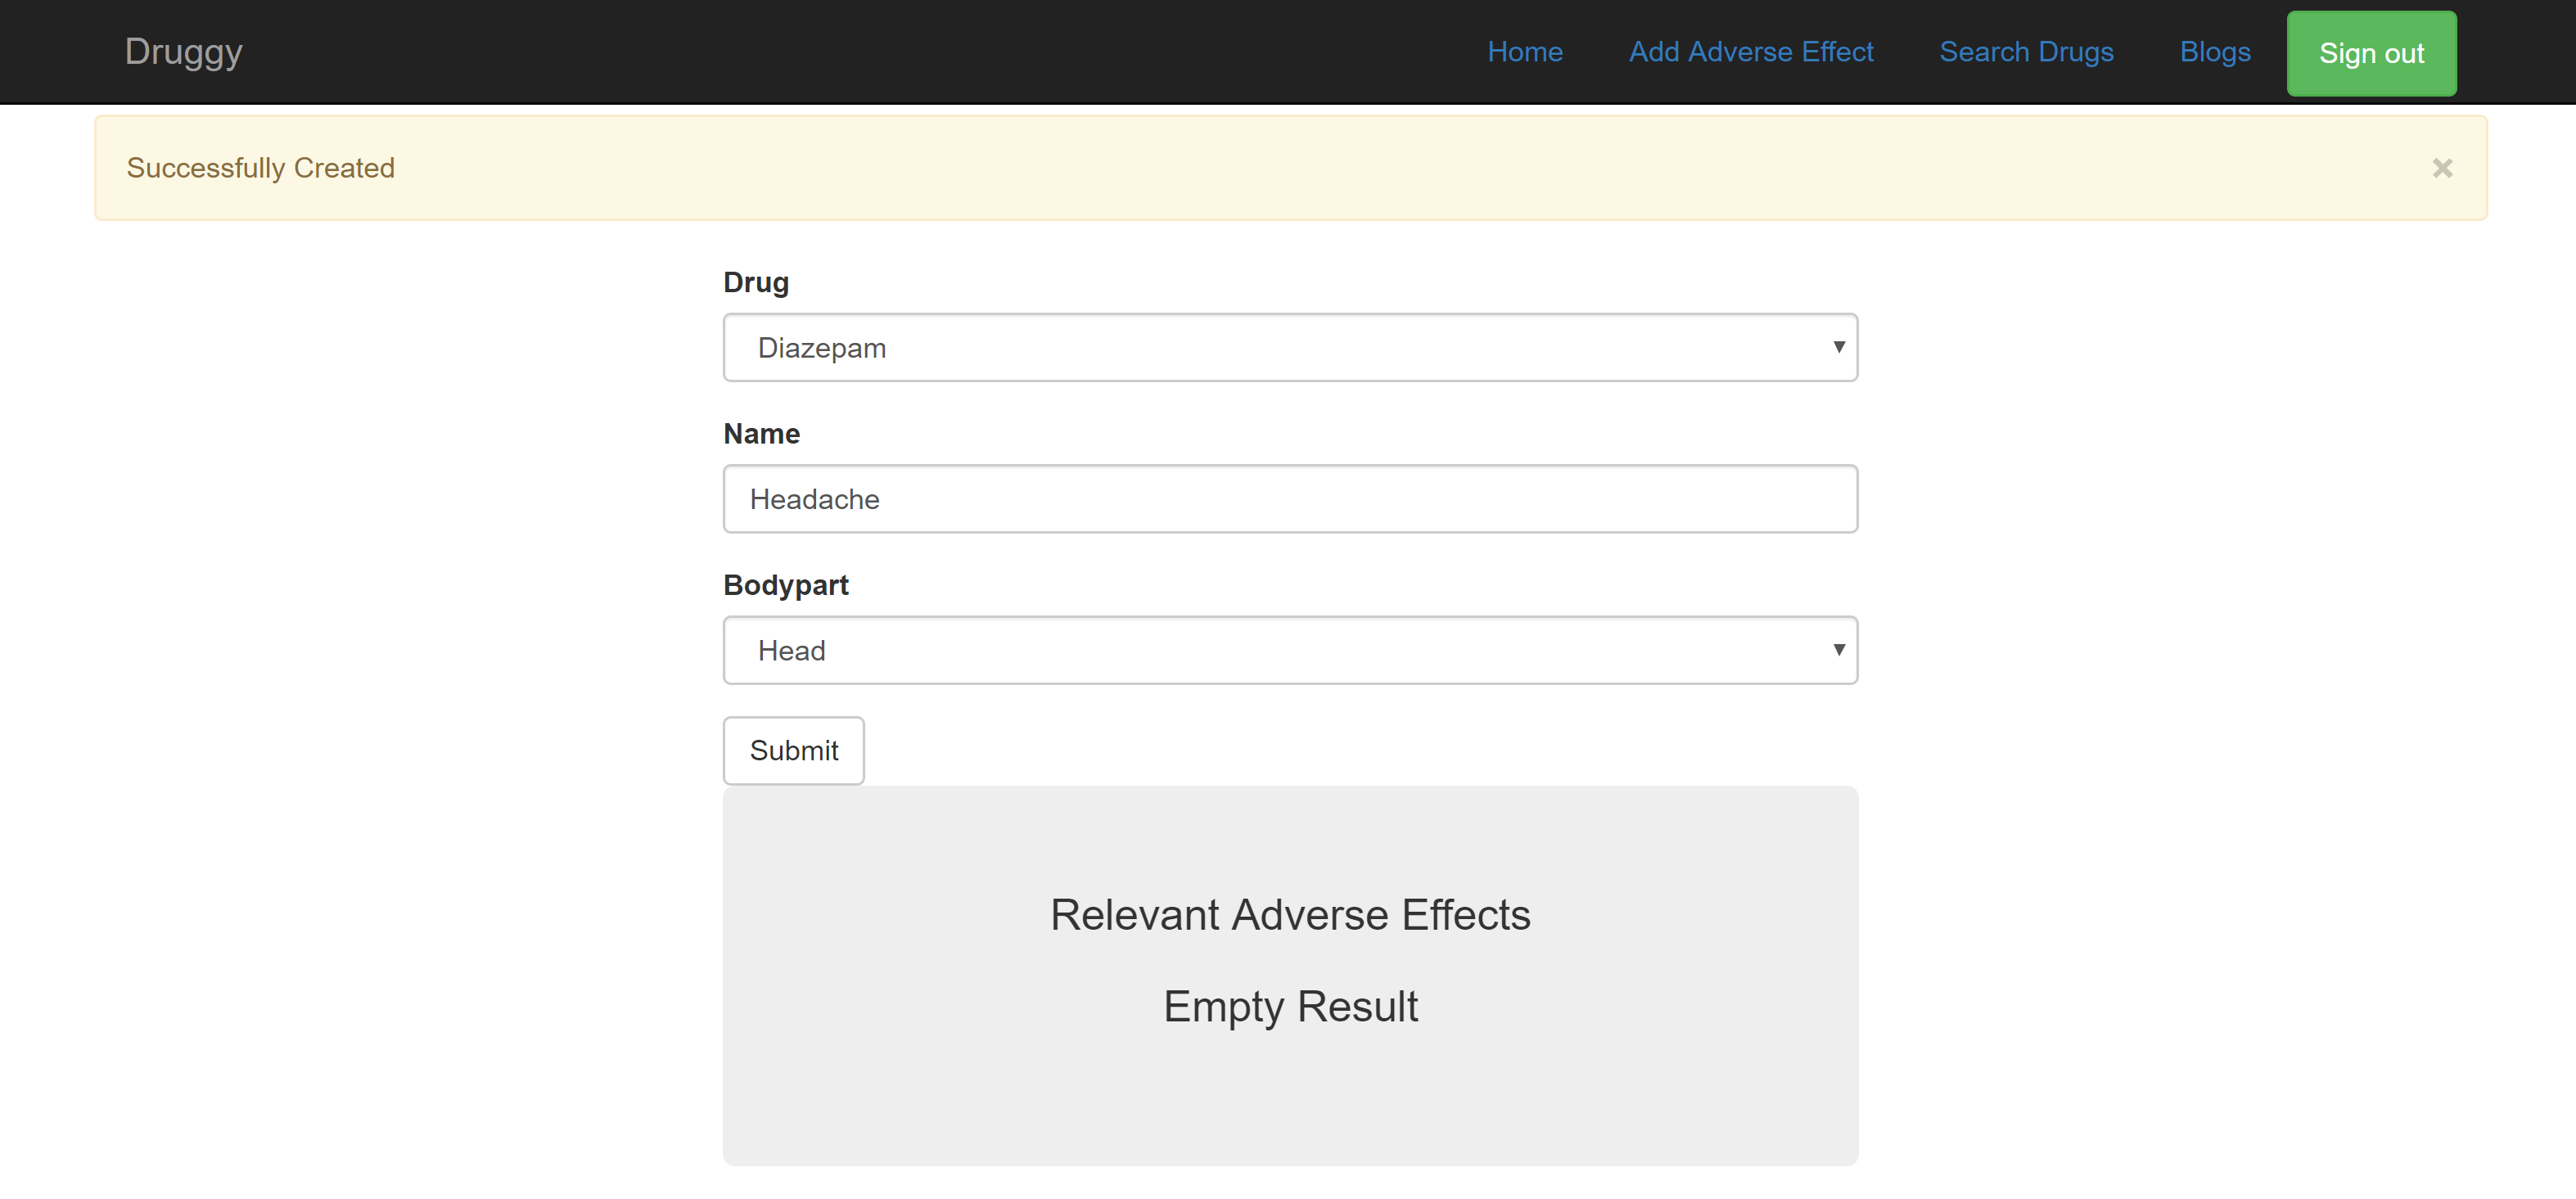
\includegraphics[width=0.8\textwidth]{scr1.png}
\end{figure}

\begin{figure}
	\centering
	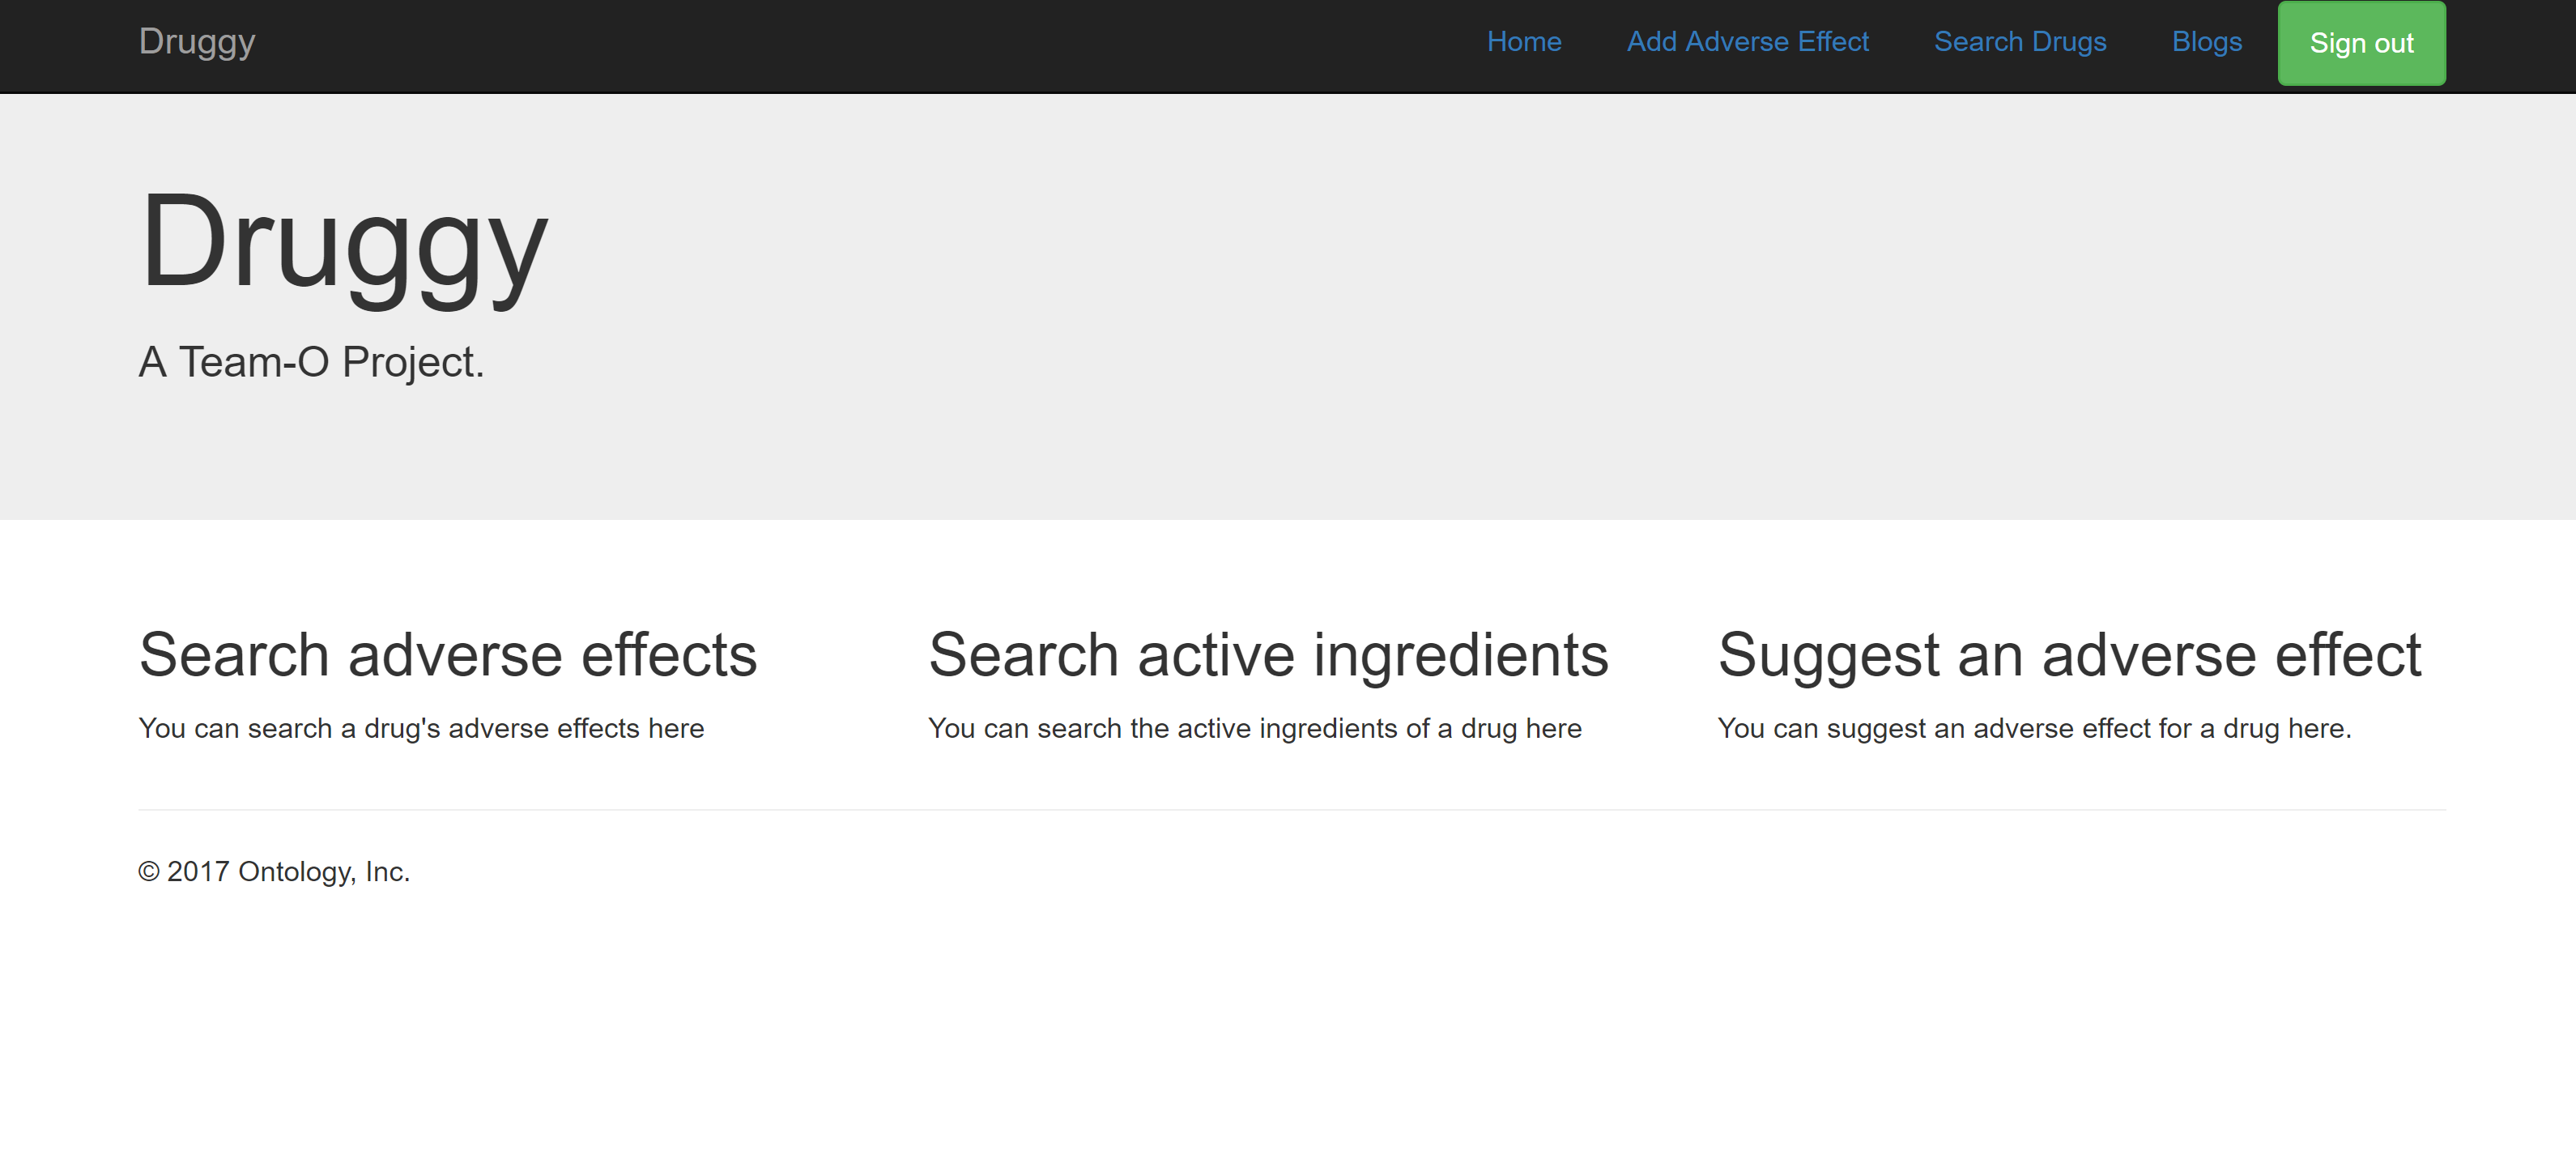
\includegraphics[width=0.8\textwidth]{scr2.png}
\end{figure}

\begin{figure}
	\centering
	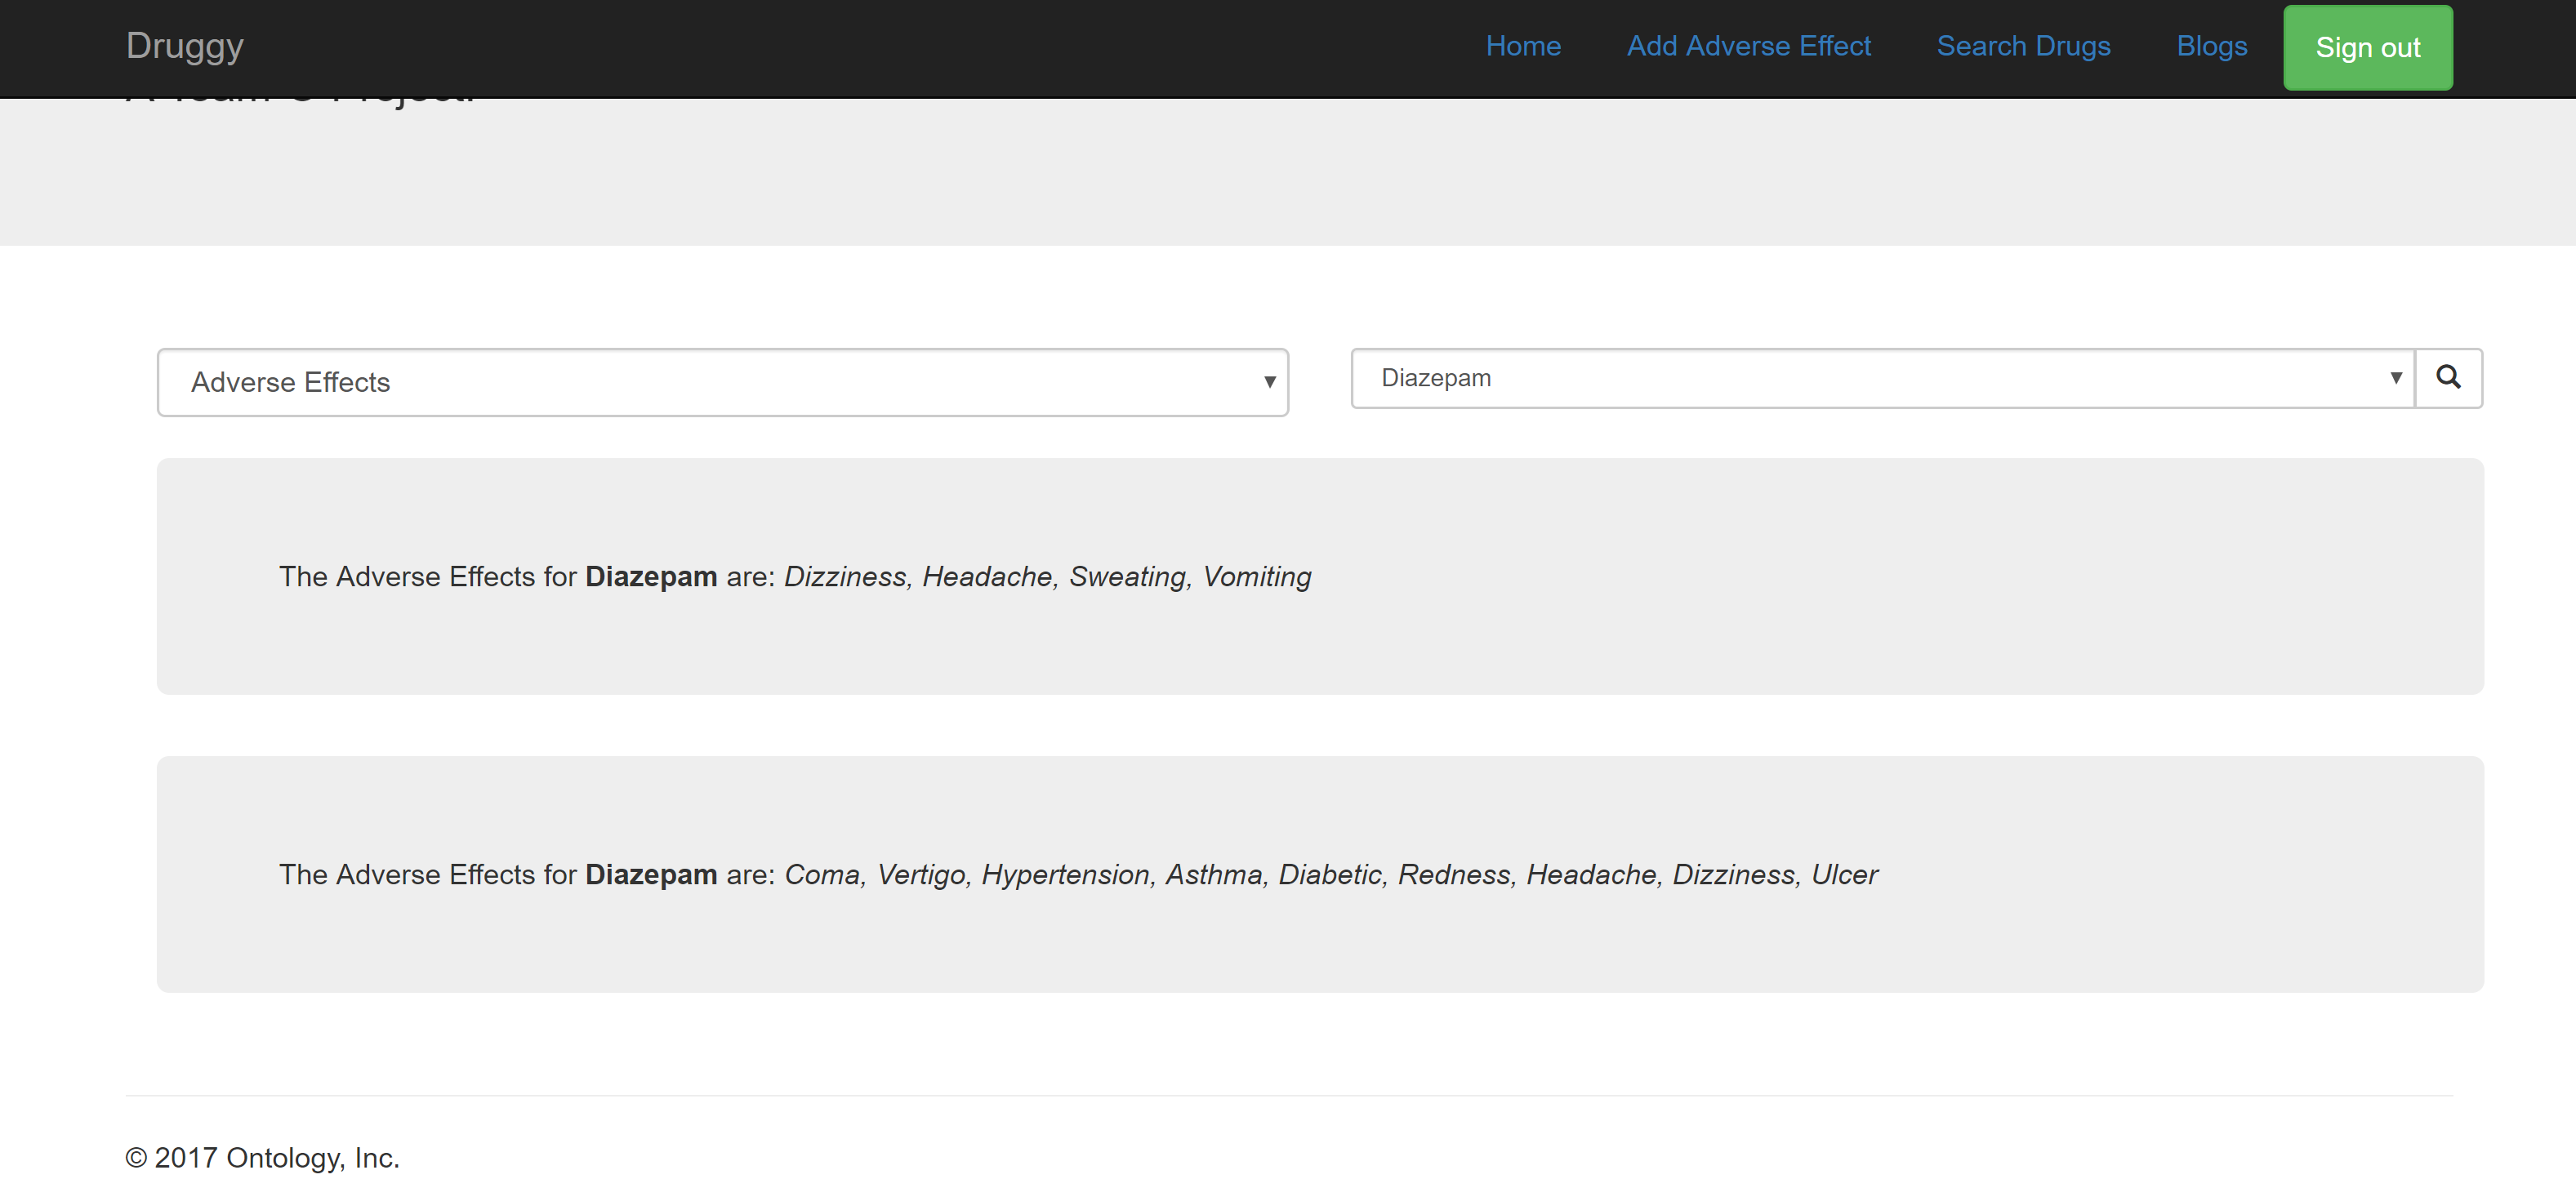
\includegraphics[width=0.8\textwidth]{scr3.png}
\end{figure}

\begin{figure}
	\centering
	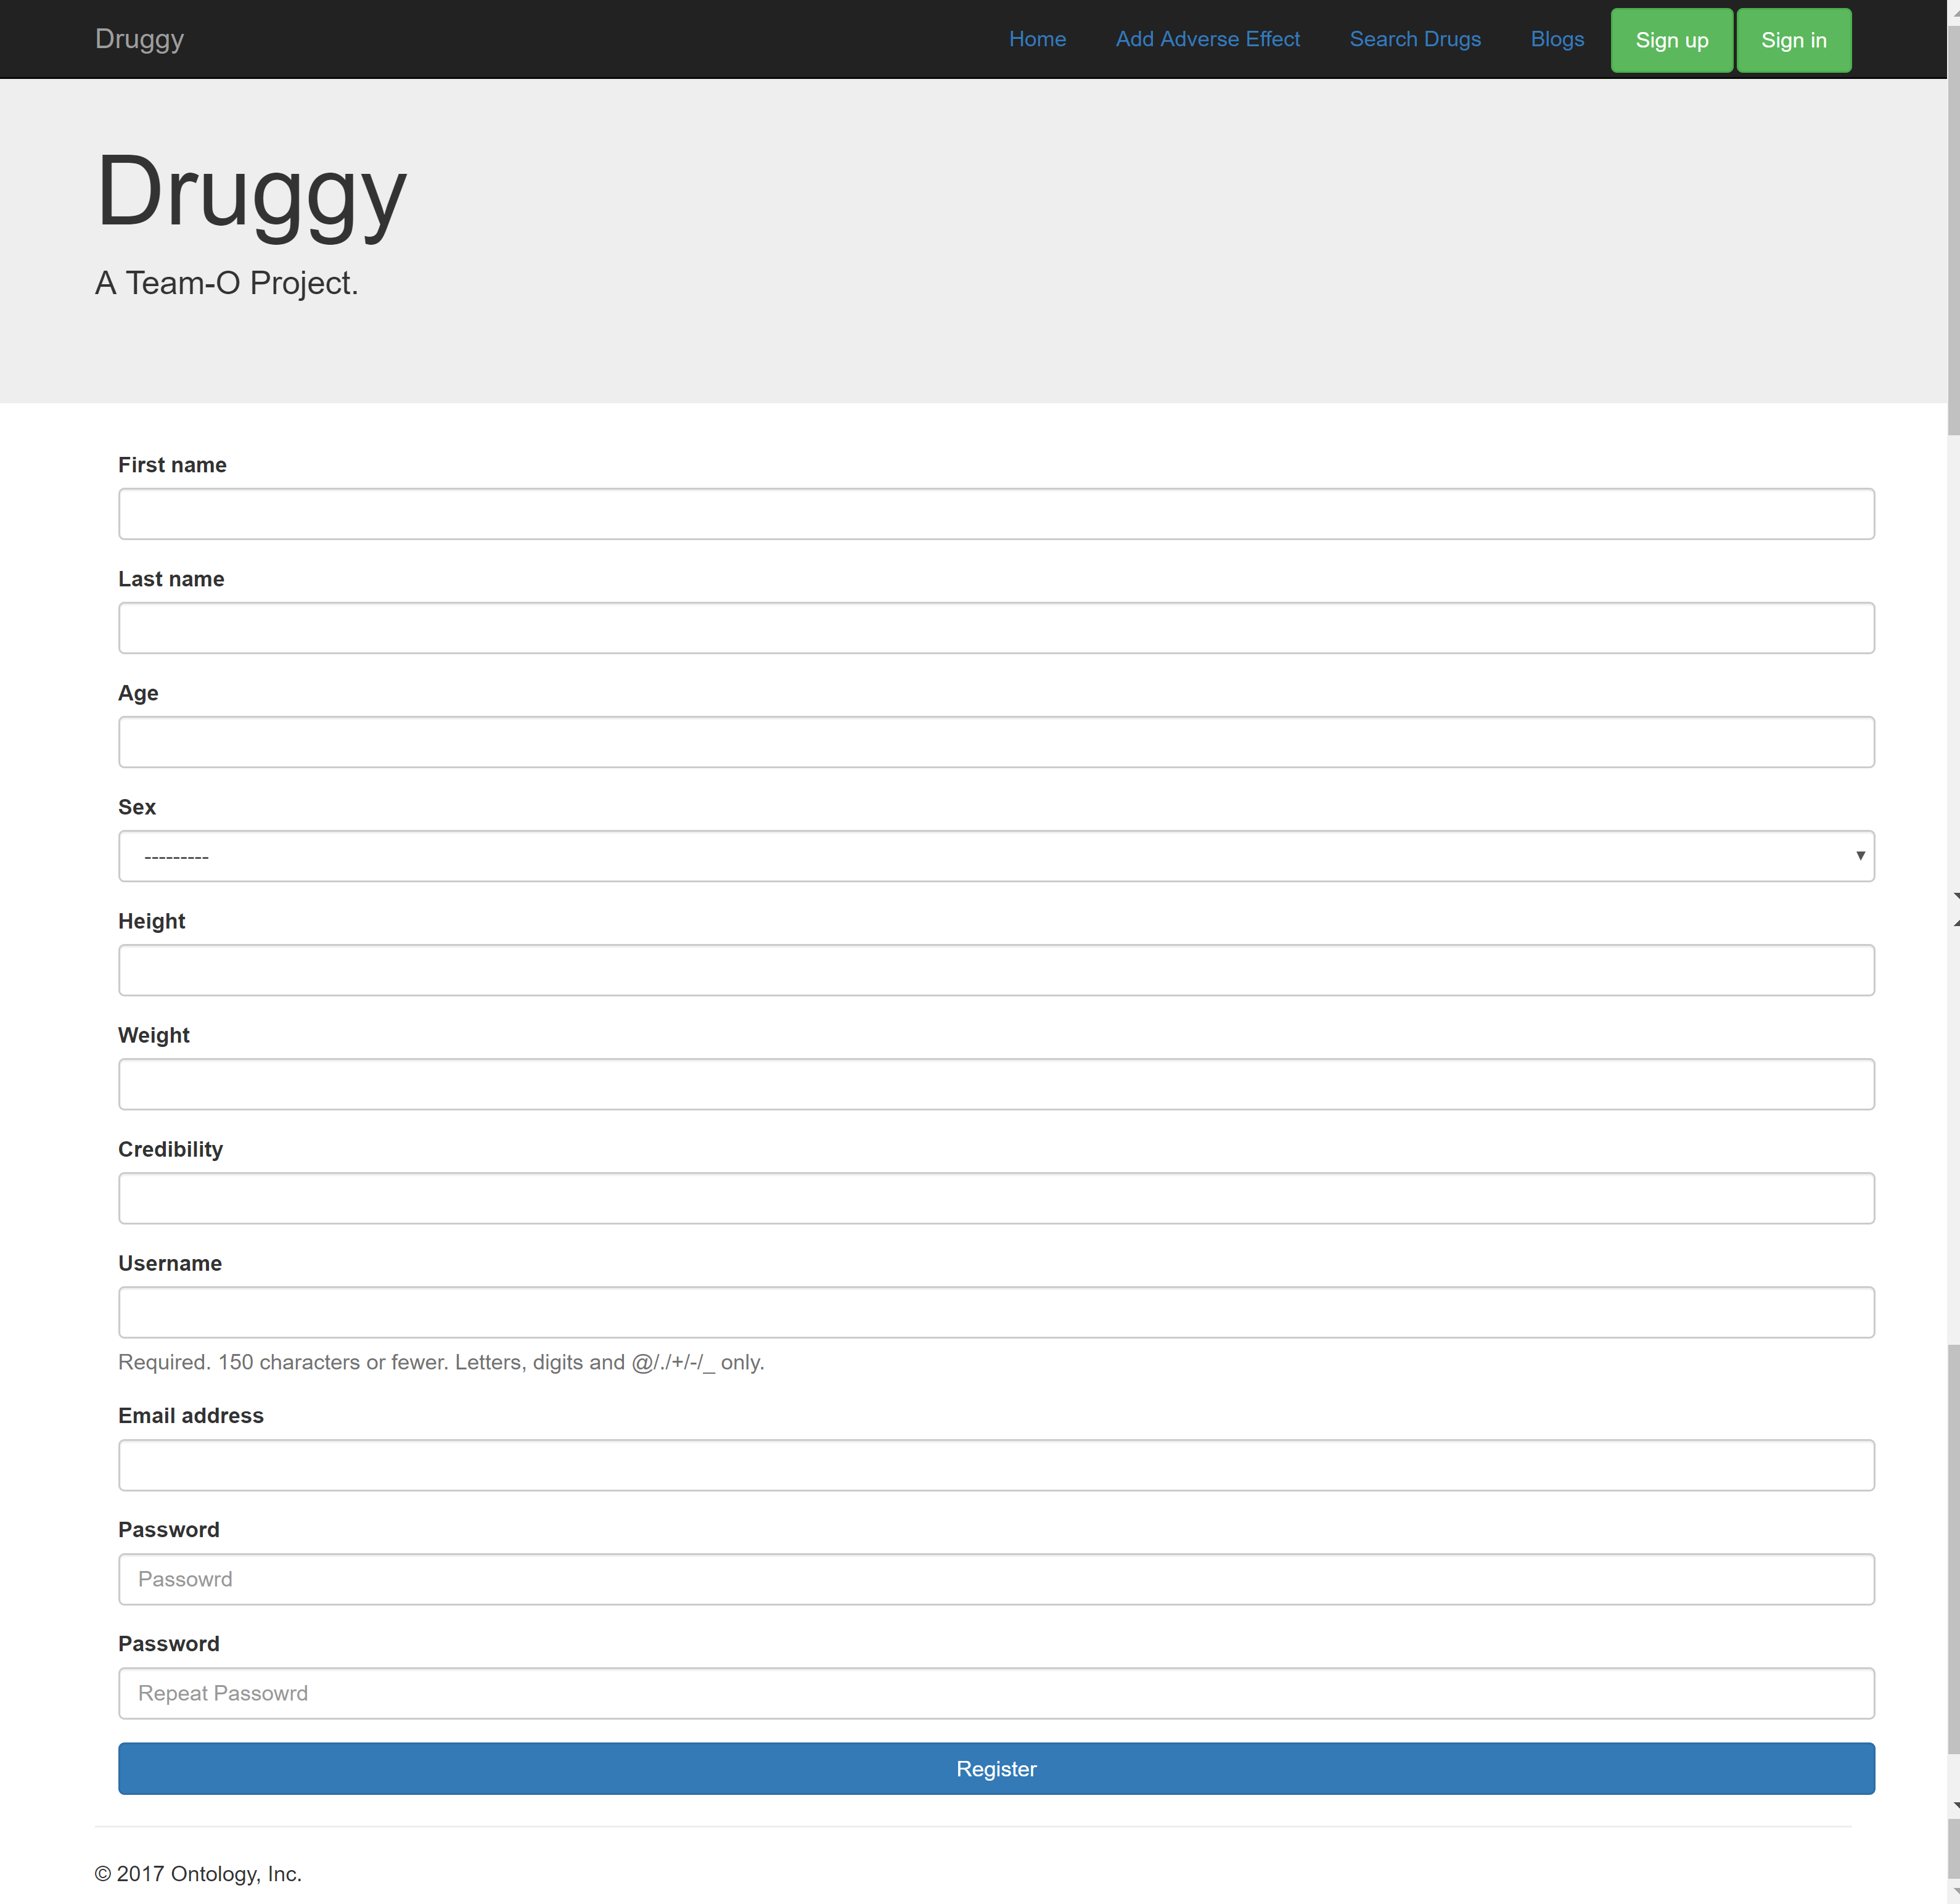
\includegraphics[width=0.8\textwidth]{scr4.png}
\end{figure}


\bibliographystyle{plain}
\bibliography{references}
\end{document} 